% Sample pages for Ceyhun Cizge Kurami

% Haluk Bingol
% v20161028

\documentclass[11pt]{amsbook}
\usepackage[turkish]{babel}

\usepackage{../Ceyhun}	% ------------------------
\usepackage{../amsTurkish}


\usepackage{lipsum}
\usepackage{graphicx}


\begin{document}



% =======================================
%\chapter{}
% ++++++++++++++++++++++++++++++++++++++
%\hPage{078}
% ++++++++++++++++++++++++++++++++++++++
% =======================================
%\section{}
% ++++++++++++++++++++++++++++++++++++++
\hPage{078}
% ++++++++++++++++++++++++++++++++++++++
% =======================================
%\section{}
% =======================================
%\section{}
% =======================================
\subsection{EULER ÇİZGELERİ}
	Çizge kuramı, doğuşunu ve ilk gelişimini bir yerde 
	bulmacalara borçludur. Bunlardan en başta geleni 
	de ' Königsberg Köprüleri'  diye adlandırılanıdır. 
	Königsberg (bugünkü Kaliningrad) kentindeki Pregel 
	ırmağında, Şekil \ref{fig:2.5.1} de gösterildiği gibi, iki 
	ada ve bu adaları birbirlerine ve kıyılara 
	bağlayan yedi köprü vardır. Sorun A, B, C ve D 
	\begin{figure}[h] \centering 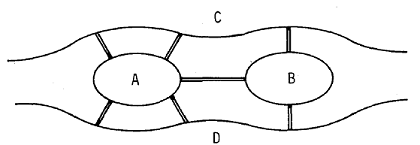
\includegraphics[width=0.9\textwidth,keepaspectratio=true]{images/ceyhun-078-fig01}\caption{ Königsberg Köprüleri.} \label{fig:2.5.1} \end{figure}
	ile gösterilen herhangi bir kara parçasından 
	başlayarak ve yeryuvarlağının çevresinde dolanmadan 
	ya da uçmadan, bu yedi köprünün her birinden yalnız  
	bir kez geçerek başlangıç yerine geri gelmekti. 
	Euler bu bulmacanın çözümünü ararken, bugün Euler 
	çizgesi diye adlandırdığımız çizgelerin 
	özelliklerini ortaya koyarak, çizge kuramının da 
	temellerini atmış oldu. Königsberg köprülerinin 
	çözümünü biraz erteleyerek, önce Euler çizgelerinin 
	tanımını verelim.
% =======================================
%\subsubsection{}
% =======================================================
\end{document}  
%==== templates ====

%==== environments ====

%\begin{figure}[htb]
%	\centering
%	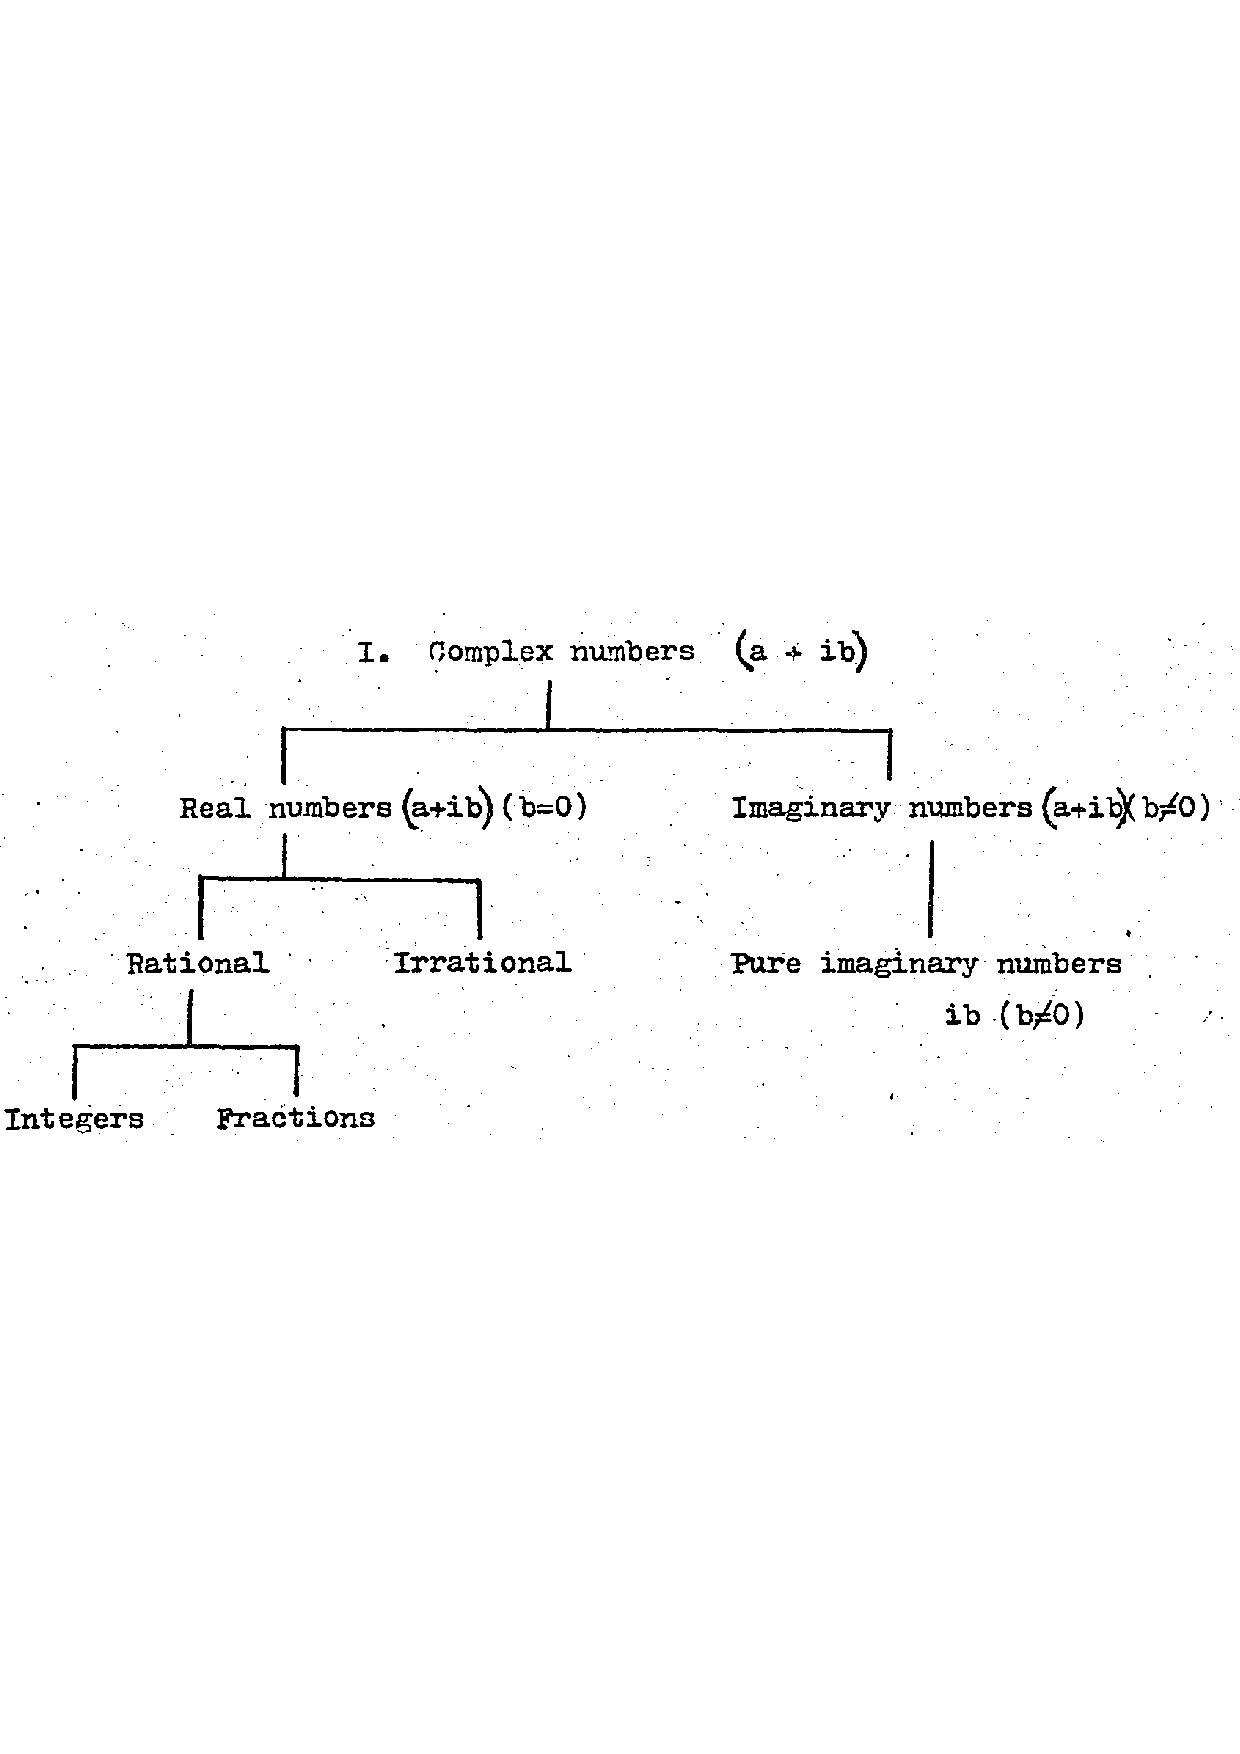
\includegraphics[width=0.9\textwidth]{images/SD-1-1p15A}
%	\caption{Classification of complex numbers}
%	\label{fig:classificationOfComplexNumbersA}
%\end{figure}

%\begin{center}
%\begin{tabular}{cc}
%\end{tabular}
%\end{center}

%\begin{exmp}
%\begin{hSolution}
%\end{hSolution}
%\end{exmp}

%\begin{hEnumerateAlpha}
%\end{hEnumerateAlpha}

%\begin{hEnumerateRoman}
%\end{hEnumerateRoman}

%$
%\begin{bmatrix}
%\end{bmatrix}
%$

%\frac{aaaa}{bbb}
%\frac{a_{n}}{b_{n}}
%\left( aaaa \right)
%\Longrightarrow

%\begin{multicols}{2}
%	bb
%\columnbreak
%	aa
%\end{multicols}
